\subsection{Comunicazione e risoluzione di anomalie}
Un'anomalia corrisponde a una mancanza di regolarità rispetto alle procedure previste per le diverse attività. Nel corso delle attività di verifica si possono riscontrare diverse anomalie. Esse potranno riguardare:
\begin{itemize}
	\item Violazione delle \textit{Norme di Progetto v1.0.0};
	\item Uscita dal range di accettazione da parte di una delle misurazioni;
	\item Distacco rispetto ai requisiti specificati durante l'analisi dei requisiti.
\end{itemize}
Nel caso in cui il \textit{Verificatore} individui un'anomalia dovrà aprire un \gls{ticket} di segnalazione. Per la gestione completa di questi problemi si rimanda alla consultazione delle \textit{Norme di Progetto v1.0.0}.

\subsection{Procedure di controllo di qualità di processo}
La qualità dei processi è basata sul \textit{ciclo di Deming}. Tale modello è studiato per il miglioramento continuo della qualità in un'ottica a lungo raggio.
Il \textit{ciclo di Deming} è chiamato anche \textit{\gls{PDCA}} a causa delle quattro fasi che lo compongono:
\begin{itemize}
	\item \textbf{Plan:} fase di pianificazione in cui si stabiliscono gli obbiettivi e i processi necessari per raggiungerli;
	\item \textbf{Do:} fase in cui si eseguono le attività rispettando il piano;
	\item \textbf{Check:} si verificano i risultati ottenuti e si confrontano con quelli attesi dalla fase Plan;
	\item \textbf{Act:} fase in cui si rendono definitivi i processi o si procede al miglioramento degli stessi. 
\end{itemize}
Per migliorare la qualità, le quattro fasi devono ruotare costantemente, tenendo come criterio principale la qualità di processo.
\begin{figure}[h]
\centering
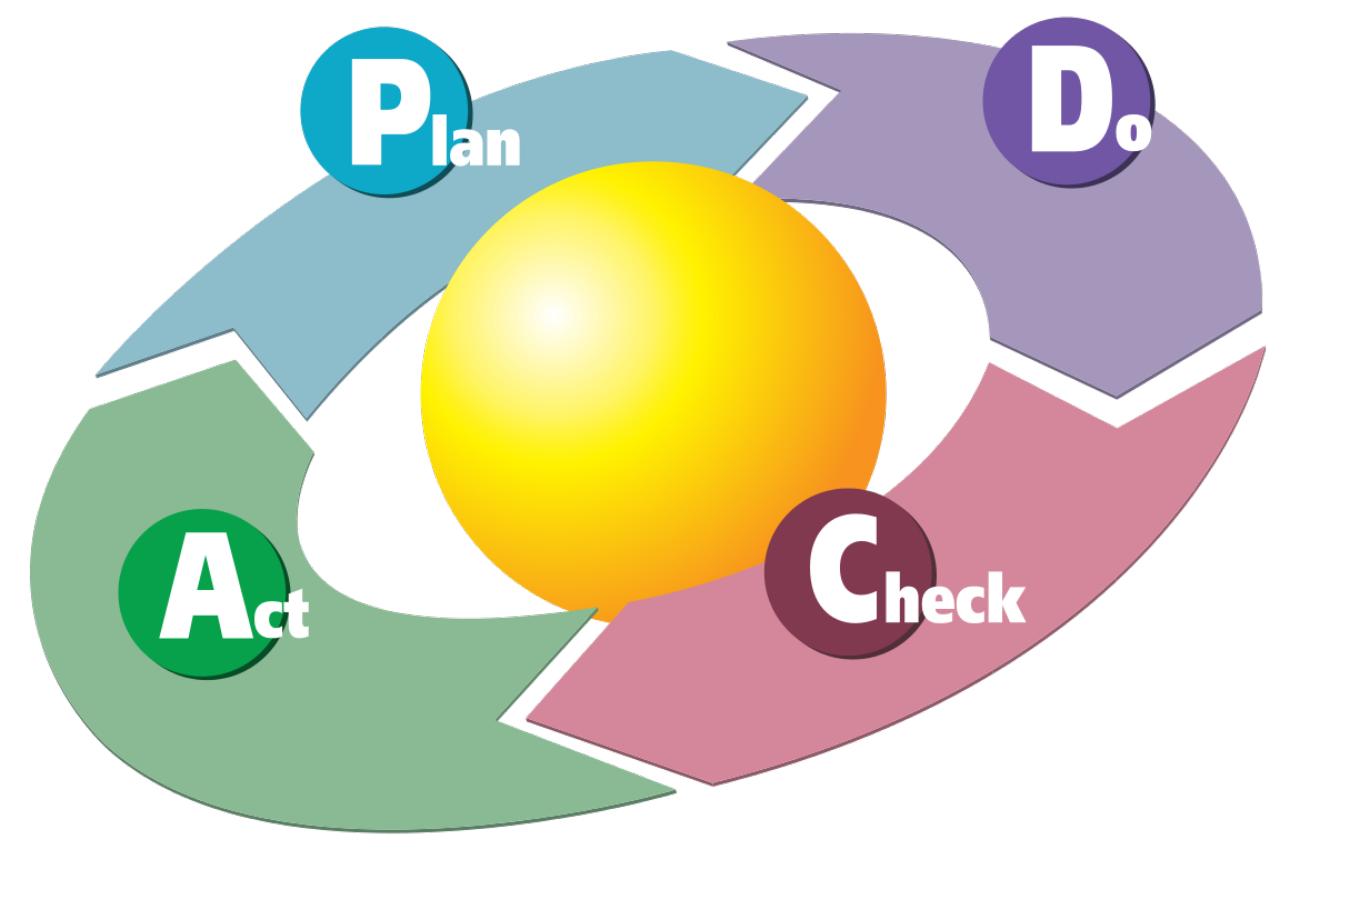
\includegraphics[width=0.7\linewidth]{img/PDCA_Cycle}
\caption[Il ciclo PDCA]{Il ciclo PDCA}
\label{fig:PDCA_Cycle}
\end{figure}

\subsection{Procedure di controllo di qualità di prodotto}
Il gruppo svolge ogni attività necessaria alla gestione del progetto in modo da migliorare la qualità del prodotto, perciò si è deciso di aderire allo standard ISO/IEC 9126\footnote{Per una descrizione dettagliata dello standard si rimanda all'appendice \ref{9126}.} al fine di garantirne il miglioramento. La norma tecnica relativa alla qualità del software si compone in quattro parti:
\begin{itemize}
	\item \textbf{Modello della qualità del software;}
	\item \textbf{Metriche per la qualità esterna;}
	\item \textbf{Metriche per la qualità interna;}
	\item \textbf{Metriche per la qualità in uso.}
\end{itemize}

